\documentclass{article}
\usepackage{graphicx}
\usepackage{amsmath}
\usepackage{listings}
\usepackage{caption}
\usepackage[hidelinks]{hyperref}
\setlength{\parindent}{0pt}


\begin{document}

    \begin{titlepage}
    \vbox{ }
    \vbox{ }
    \begin{center}
        % Course
        
\includegraphics[width=1\textwidth]{./images/ifi.png}\\[1cm]
        \textsc{\Large IN4050 - Introduction to Artificial Intelligence and Machine Learning}\\[0.5cm]
        \vbox{ }
        
        % Title
        { \huge \bfseries Mandatory Assignment \#1}\\[0.4cm]
        
        \large
        \emph{Author:}\\
            Kjetil K. Indrehus \\[0.9cm]
           
            \large kjetiki@ifi.uio.no \\[0.1cm]
            (username: kjetiki)
        \vfill
        
        {\large\today}
    \end{center}
\end{titlepage}
    
    \section{Usage}

    All code can by run by using the Jupyter notebook called \textit{Assignment1.ipynb} file.

    This project is developed with Python virtual environment. 
    All packages required are in the \textit{requirements.txt}.
    With VSCode, use the following guide to setup the virtual environment \url{https://code.visualstudio.com/docs/python/environments}.

    After the environment are created, you should have a \textit{.venv} directory in the root folder. 
    Make sure to select the environment when using the notebook. 

    \newpage

    \section{Exhaustive search}

    My implemented the Exhaustive Search algorithm has the following steps: 

    \begin{itemize}
        \item Creating variables for storing the best solutions.
        \item Iterate over each city, and make that city the starting point. 
        \begin{itemize}
            \item Generate all possible permutations of the list of cities without the starting city. Each permutation is the \textit{middle route} and does not contain the end and the start city.
            \item For each permutation, create a route by taking the starting city + the \textit{middle route} + start city again. The length of the route should be 6 or 10 cities depending on how many cities are allowed in the route.
            \item Calculate the distance for the route
            \item If the distance is lower, set the route as the best route. 
        \end{itemize}
    \end{itemize}


    \subsection{Shortest route for 10 cities}

    The following route was the shortest for 10 cities: 
    \[
    \begin{aligned}
        \text{Copenhagen} \to \text{Hamburg} \to \text{Brussels} \to \text{Barcelona} \to \text{Belgrade} \to\\
        \text{Istanbul} \to \text{Bucharest} \to \text{Budapest} \to \text{Berlin} \to \text{Copenhagen}
    \end{aligned}
    \]

    The total time it took was: \textbf{0:00:10.141496} (10.141496 seconds)

    This image shows the route:

    \begin{figure}[h!]
        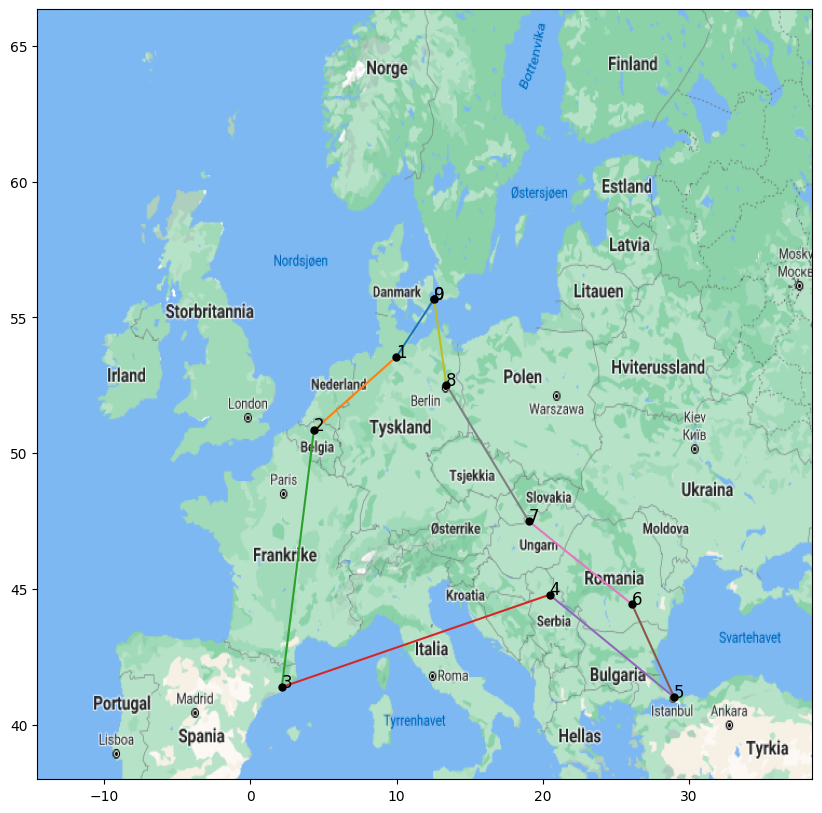
\includegraphics[width=7cm]{images/exhaustive_search_result_10_cities.png}
        \centering
    \end{figure}

    \newpage

    \subsection{Approximation for 24 cities}

    By running the code multiple times, I found out the following: 

    \begin{enumerate}
        \item 6 cities $\to$ 0:00:00.001407 $\to$ $P = 6! = 720$ routes to be checked 
        \item 8 cities $\to$ 0:00:00.115680 $\to$ $P = 8! = 40320$ routes to be checked 
        \item 9 cities $\to$ 0:00:00.915401 $\to$ $P = 9! = 362880$ routes to be checked 
        \item 10 cites $\to$ 0:00:10.072342 $\to$ $P = 10! = 3628800$ routes to be checked 
    \end{enumerate}

    I also tried with 12 cities, but it took more then 3 minutes. Clearly the growth is exponential with the permutations done for each route. 

    With 24 cites, there are $24! = 6,204484017*10^{23}$ possible routes!
    To approximate how long it would have taken for all the routes, I check how long it takes to generate one permutation and check it: 

    \[
    \text{Time per permutation}_n = \frac{\text{Total time}}{n!}
    \]

    For each test, I calculate how long it took for each permutation: 

    \[
    \text{Time per permutation for 6 cities} = \frac{0.001407}{720} \approx 1.9542 \times 10^{-6} \text{ s/route}
    \]

    \[
    \text{Time per permutation for 8 cities} = \frac{0.115680}{40320} \approx 2.8696 \times 10^{-6} \text{ s/route}
    \]

    \[
    \text{Time per permutation for 9 cities} = \frac{0.915401}{362880} \approx 2.5236 \times 10^{-6} \text{ s/route}
    \]

    \[
    \text{Time per permutation for 10 cities} = \frac{10.072342}{3628800} \approx 2.7766 \times 10^{-6} \text{ s/route}
    \]

    With this, I assume that each permutation will take the average amount of time to generate a permutation: \[2.5310\times10^{-6} \text{ s/route} \]
    Note that this might not always be correct, but I think this is a good way to approximate how long it would have taken for 24 cities. 

    Now, using this average, all me need to do is multiply the amount of permutations with the average time for each permutation to be generated: 

    \[
    \begin{aligned}
        \text{Total Time} &= 6.204484017 \times 10^{23} \times 2.5310\times10^{-6} \text{ s/route} \\
                          &= 1.570354905 \times 10^{18} \text{ s}
    \end{aligned}
    \]

    To make the approximation more readable, I used a python library. 
    It has a function to make seconds into a more readable format. Link to docs: 
    \url{https://humanfriendly.readthedocs.io/en/latest/api.html#humanfriendly.format_timespan} \newline

    Using the function to get the total time in a readable format, shows how long time 24 cities with exhaustive search would have taken: \textbf{49932428552 years, 18 weeks and 1 day}.




\end{document}